\documentclass[aspectratio=169]{beamer}
\usetheme{default}

\usepackage[utf8]{inputenc}
\usepackage[ngerman]{babel}
\usepackage{graphicx}
\usepackage{csquotes}

\usepackage{lmodern}

%\usepackage{scrextend}
%\changefontsizes{18pt}

\usepackage[
backend=biber,
style=authoryear-ibid,
%sorting=ynt
]{biblatex}
\addbibresource{gravitropismus-bibliography.bib}

\author{Alexandra Smirnova}

\title{Präsentation zur Seminararbeit \hyphenquote{ngerman}{Gravitropismus}}
\subtitle{W-Seminar Biologie}

%\title{\hyphenquote{ngerman}{Gravitropismus}}
%\subtitle{Präsentation zum W-Seminar Biologie}

%\logo{}

%\institute{}

\date{19. Dezember 2018}

%\subject{}

\setbeamercovered{transparent}
%\setbeamertemplate{navigation symbols}{}
\setbeamertemplate{section in toc}[sections numbered]
\setbeamertemplate{subsection in toc}[subsections numbered]
\setbeamertemplate{caption}[numbered]


\useoutertheme{infolines}

\begin{document}
	\maketitle
	
	\begin{frame}
		\frametitle{Gliederung}
		\tableofcontents
	\end{frame}
	
	\section{Grundlagen von Gravitropismus}

	
	\begin{frame}
		\frametitle{Grundlagen von Gravitropismus}
		\begin{figure}[H]
			\centering 
			\includegraphics[width = 0.75\linewidth]{images/gravitrop_reagierende_Pflanze2.pdf}
			\caption{Gravitrop reagirende \emph{Arabidopsis thaliana} \parencite[5]{Masson2002}. Teilabbildung A zeigt den Zustand am Anfang, Teilabbildung B zeigt den Zustand nach vollzogener gravitropischer Reaktion. \label{gravitrop_reagierende_Pflanze}}
		\end{figure} 
	\end{frame}
	
	\subsection{Arten von Gravitropismus}
	
	\begin{frame}
		\frametitle{Arten von Gravitropismus}
		1) Positiv gravitrop - zur Schwerkraftquelle hin (nach unten zur Erdmitte)
		
		2) Negativ gravitrop - von der Schwerkraftquelle entgegengesetzt (nach oben)
		
		3) Transversalgravitrop - entweder horizontal oder quer nach unten in einem bestimmten Winkel 
		
	\end{frame}
	
	\subsection{Prozess der gravitropischen Krümmung}
	
	\begin{frame}
		\frametitle{Prozess der gravitropischen Krümmung}
		
		1) Reizaufnahme bei Pflanzen
		
		2) Signaltransduktion
		
		3) Differenzielles Wachstum
		
	\end{frame}
		
	\subsubsection{Reizaufnahme bei Pflanzen}
		
	\begin{frame}
		\frametitle{Reizaufnahme bei Pflanzen}
		\begin{figure}[H]
			\centering 
			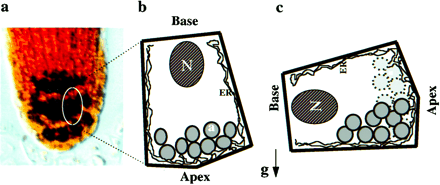
\includegraphics[width = 0.75\linewidth]{images/Statolithen2.png}
			\caption{Statolithen \parencite[345]{Chen1999}. Teilabbildung a zeigt eine Mikroskopaufnahme von Statolithen bei \emph{A. thaliana}. Teilabbildungen b und c zeigen die gravitrope Wirkungsweise von Statolithen, die auf Umlagerung der Amyloplasten bei Veränderung des Schwerkraftvektors beruht. \label{Statolithen}}
		\end{figure} 
	\end{frame}

\begin{frame}
\frametitle{Reizaufnahme bei Pflanzen}

1) Reize durch Statolithen (Amyloplasten, die aus Stärke bestehen)

2) Statolithen in Statocysten (Statenchyme bei größeren Mengen der Statolithen) in Wurzelspitzen und Innenzellschichten der Sprossachse

3) Statolithen auf der Membran des endoplasmatischen Retikulums (ER)

\end{frame}

\begin{frame}
\frametitle{Reizaufnahme bei Pflanzen}

 \begin{figure}[H]
	\centering 
	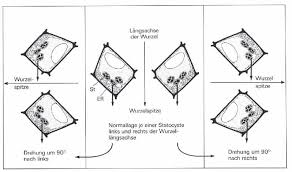
\includegraphics[width = 0.55\linewidth]{images/Graviperzeption.jpeg}
	\caption{Querlegen einer Wurzel der Kresse (\emph{Lepidium sativum}). Es erfolgt eine Graviperzeption, in der die Entlastung des Drucks der Membran des ER zu erkennen ist \parencite[533]{Luettge}. \label{Graviperzeption}}
\end{figure} 

\end{frame}
			
	\subsubsection{Signaltransduktion}
		
	\begin{frame}
		\frametitle{Signaltransduktion}
		
		1) Signalübermittlung durch Kontakt zwischen Amyloplasten und ER (gravisensorische Transduktion)
		
		1. Funktion des Calciums:
		
	    1.1 %\ce{Ca^{2+}}-Efflux durch Druck der Amyloplasten auf die ER-Membran 
		
		1.2 Erhöhung der lokalen %\ce{Ca^{2+}}-Konzentration im Cytoplasma
		
		2. Funktion des elektrischen Feldes:
		
		2.1 Elektrisches Feld (um die Wurzel herum) durch apoplastischen Strom (Ionenbewegung) 
		
		2.2 Bei horizontaler Lage der Pflanze: Änderung des elektrischen Feldes durch die veränderte Richtung des apoplastischen Stroms
		
		2) Aufnahme des entstandenen Signals (durch die Graviperzeption) in der Streckungszone hinter der Wurzelspitze
		
		3) Einsetzung der Krümung beim Ankommen des Signals (ungleiches Wachsen der Flanken)
		
		
		
	\end{frame}
			
	\subsubsection{Differenzielles Wachstum}
		
	\begin{frame}
		\frametitle{Differenzielles Wachstum}
		
		Funktion der Auxine und Gibberelline
		\begin{figure}[H]
			\centering 
			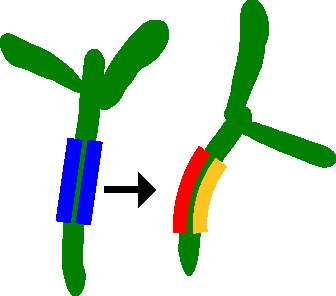
\includegraphics[width = 0.4\linewidth]{images/newdiff.pdf}
			\caption{Flanken wachsen ungleich nach der Signaltransduktion. Linkes Bild: Flanken gleich groß (blau); rechtes Bild: unterschiedliche Größe der Flanken (rot und orange).}
		\end{figure} 
	\end{frame}

	\begin{frame}
\frametitle{Differenzielles Wachstum}

 1) Funktion der Auxine (hier: Indolessigsäure): 
 
 1. Synthesierung des Auxins im Apikalmeristem
 
 2. Bewegung der Auxine vom Apikalmeristem bis zur Streckungszone für die Stimulierung des Zellwachstums
 
 2.1 Stimulierung der Protonenpumpe für die Ansäuerung der Zellwand 
 
 2.2 Aktiwierung der Expansine für die Auflockerung der Zellwand
 
 2.3 Erhöhte Ionenaufnahme in der Zelle und damit Erhöhung des osmotischen Drucks
 
 2.4 Mödliche Ausdehnung der Zellwand
 
 2) Funktion der Gibberelline:
 
 2.1 Zusammenwirken der Gibberelline mit Auxin bei der Zellstreckung
 
 2.2 Aktivierung der Enzyme für die Auflockerung der Zellwand und für den erleichterten Eintritt der Expansinen dahin
 
 
 
 
\end{frame}
	
	\section{Experimenteller Nachweis von Gravitropismus bei \protect\emph{Lepidium sativum}}
	
	\begin{frame}
		\frametitle{Experimenteller Nachweis von Gravitropismus bei \protect\emph{Lepidium sativum}}
		
		1) Methoden
		
		1.1 Pflanzen, Materialien und Geräte
		
		1.2 Versuchmethodik
		
		2) Durchführung und Ergebnisse
		
		2.1 Vorbereitung 
		
		2.2 Ankeimen 
		
		2.3 Klinostat-Experiment mit Pflanzengruppe 2
		
		2.4 Ausrichtungs-Experiment mit Pflanzengruppe 3-5
		
		3) Diskussion
		
	\end{frame}	
	
	\subsection{Methoden}
	
	\begin{frame}
		\frametitle{Methoden}
		\begin{figure}[H]
			\centering 
			\includegraphics[width = 0.5\linewidth]{images/IMG_1044.JPG}
			\caption{Vorbereitung des Experiments und vollständig aufgebautes Klinostat.\label{Klinostat2}}
		\end{figure}
		
	\end{frame}
	
	\subsubsection{Pflanzen, Material und Geräte}

	\begin{frame}
		\frametitle{Pflanzen, Material und Geräte}
		1) Pflanzen - \protect\emph{Lepidium sativum}
		
		2) Klinostat
		
		3) Weitere Materialien: Anzuchtbehälter, Säckchen aus Stoffstück, Plastiktüte, Messzylinder aus Plastik, diverse Gegenstände (z.B. Holzwürfel) 
	\end{frame}
	
	\subsubsection{Versuchsmethodik}
	
	\begin{frame}
		\frametitle{Versuchsmethodik}
		1) Pflanzengruppe 1: Kontrollgruppe
		
		2) Pflanzengruppe 2: Säckchen am Klinostat
		
		3) Pflanzengruppe 3: Anzuchttopf kopfüber
		
		4) Pflanzengruppe 4: Anzuchttopf horizontal am Boden
		
		5) Pflanzengruppe 5: Anzuchttopf mit Winkel zum Boden 
		
	\end{frame}
	
	\subsection{Durchführung und Ergebnisse}
	
	\begin{frame}
		\frametitle{Durchführung und Ergebnisse}
		
		1) Versuchstag 1 (28.05.2018): Vorbereitung
		
		2) Versuchstage 2–4 (29.–31.05.2018): Ankeimen
		
		3) Versuchstage 4–5 (31.–01.06.2018): Klinostat-Experiment mit Pflanzengruppe 2
		
		4) Versuchstage 6–7 (02.–03.06.2018): Ausrichtungs-Experiment mit Pflanzengruppe 3-5
	\end{frame}
	
	\subsubsection{Vorbereitung, Ankeimen}
	
	\begin{frame}
		\frametitle{Vorbereitung, Ankeimen}
		1) Vorbereitung (Versuchstag 1, 28.05.2018):
		
	 	1.1 Bestimmung des Ortes
			
		1.2 Vorbereiten der vier Anzuchtbehälter + Säckchen 
			
		2) Ankeimen (Versuchstage 2-4, 29.–31.05.2018):
		
		Prozess der Keimung von Kressesamen, bis zu stabil gewachsenen Sprösslingen
				
		
	\end{frame}
	
	\subsubsection{Klinostat-Experiment}
	
	\begin{frame}
		\frametitle{Klinostat-Experiment}
		
	\begin{figure}[H]
	\centering
	\includegraphics[width=0.5\linewidth]{images/IMG_1083.JPG}
	\caption{Sprossen vor Beginn des Klinostat-Experiments.\label{Foto 1}}	
	\end{figure}	
	
	\end{frame}

\begin{frame}
\frametitle{Klinostat-Experiment}

\begin{figure}[H]
	\centering		 \includegraphics[width=0.5\linewidth]{images/IMG_1073.JPG}	\caption{Sprossen nach Abschalten des Klinostats.\label{Foto 2}}
	
\end{figure}

\end{frame}


	\subsubsection{Ausrichtungs-Experiment}
	
	\begin{frame}
		\frametitle{Ausrichtungs-Experiment}
	Ausrichtungs-Experiment mit Pflanzengruppe 3-5 (Versuchstage 6-7, 02.–03.06.2018):
	
	1) Gruppe 3 parallel zum Boden
	
	2) Gruppe 4 kopfüber
	
	3) Gruppe 5 im Winkel von ca. %\ang{45}
	
\end{frame}
	

\begin{frame}
\frametitle{Ausrichtungs-Experiment}
\begin{figure}[H]
\centering
\includegraphics[width=0.5\linewidth]{images/A4/IMG_1104.JPG}
\caption{Sprossen vor Neuausrichtung.\label{A41}}	
\end{figure}
\end{frame}

\begin{frame}
\frametitle{Ausrichtungs-Experiment}
\begin{figure}[H]
\centering
\includegraphics[width=0.5\linewidth]{images/A4/IMG_1396.JPG}
\caption{Sprossen am Versuchstag 7.\label{A47}}
\end{figure}
\end{frame}	
	
\begin{frame}
\frametitle{Ausrichtungs-Experiment}
\begin{figure}[H]
\centering
\includegraphics[width=0.5\linewidth]{images/A3/IMG_1102.JPG}
\caption{Sprossen vor Neuausrichtung.\label{A31}}	
\end{figure}
\end{frame}

\begin{frame}
\frametitle{Ausrichtungs-Experiment}
\begin{figure}[H]
\includegraphics[width=0.5\linewidth]{images/A3/IMG_1398.JPG}
\caption{Sprossen am Versuchstag 7.\label{A37}}
\end{figure}
\end{frame}

\begin{frame}
\frametitle{Ausrichtungs-Experiment}
\begin{figure}[H]
\centering
\includegraphics[width=0.5\linewidth]{images/A5/IMG_1101.JPG}
\caption{Sprossen vor Neuausrichtung.\label{A51}}		
\end{figure}
\end{frame}

\begin{frame}
\frametitle{Ausrichtungs-Experiment}
\begin{figure}[H]
\centering
\includegraphics[width=0.5\linewidth]{images/A5/IMG_1397.JPG}	\caption{Sprossen am Versuchstag 7.\label{A57}}
\end{figure}
\end{frame}


	
	\subsection{Diskussion und Fazit}
	
	\begin{frame}
		\frametitle{Diskussion und Fazit}
		
	1) Besprechung der Abhängigkeit des gravitropen Effekts von verschiedenen Faktoren:
	
	Sprosslänge, Stärke des Reizes, übermäßiger Reiz, Lichteinwirkung und Reizkonkurrenz
	
	2) Unberücksichtigte Faktoren:
	
	Schwankungen in pflanzlichen Hormonen, unterschiedliche Samen, unterschiedliche initiale Wachstumsphasen, Umweltfaktoren wie Druck, Temperatur und Feuchtigkeit, Einflüsse durch das Nährmedium
	
 
		
		
\end{frame}	
	

\end{document}